\chapter{Software Process}
There are different approaches for software development which were designed in order to 
facilitate the creation of software systems. Regardless of the chosen approach the 
process of software creation includes three generic phases: definition phase, 
development phase and a maintenance phase \cite{citeulike:6095377}.
The definition phase includes the initial
planning of the future system and requirements collection. Developers identify data 
need to be processed by the system, its functionality, behavior, and what are 
the constraints there are in the design and development. The development phase focuses 
on the system implementation and its testing. Developers write the system code, 
test if the system satisfies planned requirements in the behavior and and output. 
The maintenance phase focuses on the post-development activities: system deployment 
and its operational support. 

Another common part of these approaches is the use 
of a software process model and following a software method, also known as methodology.
While latter is used to primarily navigate through the development process determining
a number of functional points, designing data flow diagrams etc., the model provides 
developers with guidance about their tasks and the activities that should be undertaken 
during development. It is advocated that the use of established and well structured 
model is crucial for the complex projects in order to orchestrate collaborative effort 
of multiple teams. 

These models can be characterized by the series of distinct phases, in fact, the 
determination of phases, its ordering and the definition of the phase-transitioning 
criteria are the core model components.
Each of these phases is executed with a particular goal: some will provide a part of the 
software system, other will deliver engineering documentation or a user manual, or 
validate an existing code. Examples of such phases are the requirements collection, 
user manual writing or the coding of a functional module of the software system. 
While the methodology prescribes an ordering of carried activities, it also facilitates
a framework for estimation of needed resources, defines major milestones, and provides 
means for time and effort monitoring and management. 

In this chapter I will review major of existing software process models providing additional 
information about their derivatives and discussing their strengths and weaknesses.
The purpose of this narrowing is to present the current state of the art in software 
processes.

\section{Code-and-fix model}
According to Boehm \cite{citeulike:10002126}, the pioneering days of software development 
industry can be characterized by the application of the code-and-fix methodology
which covered full software life cycle. This model essentially consisted of two phases:
write some code and fix problems in the code. Professional programmers as well as enthusiasts 
were coding implementations of their ideas first and spent time iteratively adjusting the 
code to the requirements or errors fixing later. While being intuitively transparent, this 
approach led to the number of problems - after a number of fixes, enhancements and 
work-arounds code become unreadable and very expensive to maintain; also non-existence of
distinct testing phase allowed bugs to persist until they were revealed by the end-users.

\begin{figure}[tbp]
   \centering
   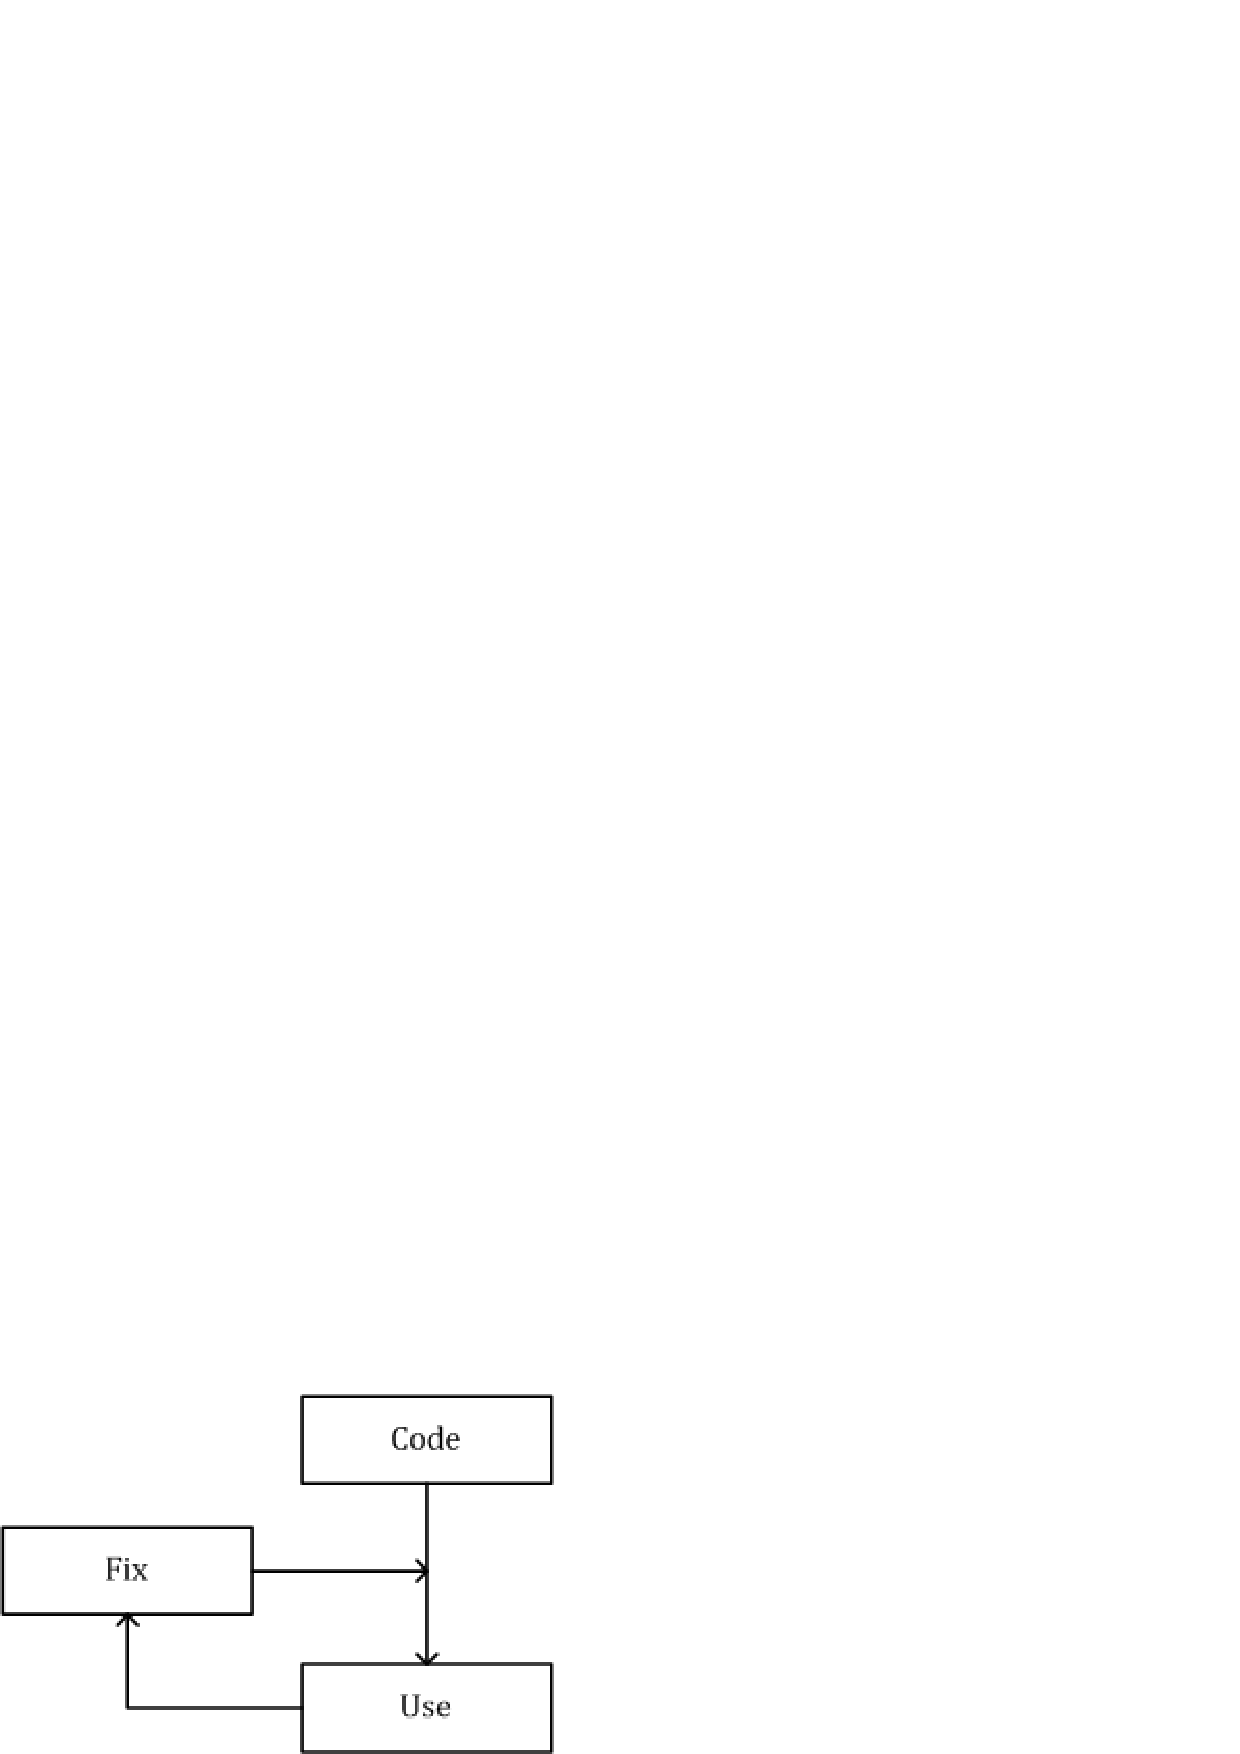
\includegraphics[height=60mm]{model_00_code_and_fix}
   \caption{The code-and-fix model \cite{citeulike:10002126}.}
   \label{fig:code_fix_model}
\end{figure}

\section{Stagewise model}
Through the experience with code-and-fix approach the need for requirements collection and 
for design phase prior to coding become evident as well as the need of structured 
testing and evaluation. The recognition these needs by the industry and the first experiences
with development of large software systems such as Semi Automated Ground 
Environment \cite{citeulike:10004001} \cite{citeulike:10004037} led to the development 
of stagewise software model by Benington (1956) \cite{citeulike:10004032}. 
This model consisted of a number of stages:
\begin{itemize}
 \item Operational plan
 \item Operational specifications
 \item Coding specifications
 \item Coding
 \item Parameter testing
 \item Assembly testing
 \item Shakedown
 \item System evaluation
\end{itemize}
These stages were streamlined as a sequential process - every completed stage created a
grounds for its successor. While seem to be naive, this formalization of the process was a 
significant breakthrough at the time. Soon it was recognized, that this unidirectional process
doesn't stipulate what to do if the rework of previous stage(s) is necessary - there was 
no formalization of such iterations and the revision of the model was requested.

\section{Waterfall model}
The Waterfall model is probably the oldest and the most influential of existing software 
process models and it is very popular in the domain of development of large and 
complex software systems. 
This model is a refinement of a stagewise model and its 
original version is credited to Royce (1970) \cite{citeulike:9982731}. There were two 
changes from the predecessor - first was a recognition of the feedback loops between 
stages and its limitation to successive stages only - in order to exclude expensive
cross-stage rework, while the second change was the inclusion of a prototyping stage
\cite{Boehm95anchoringthe}.

\begin{figure}[tbp]
   \centering
   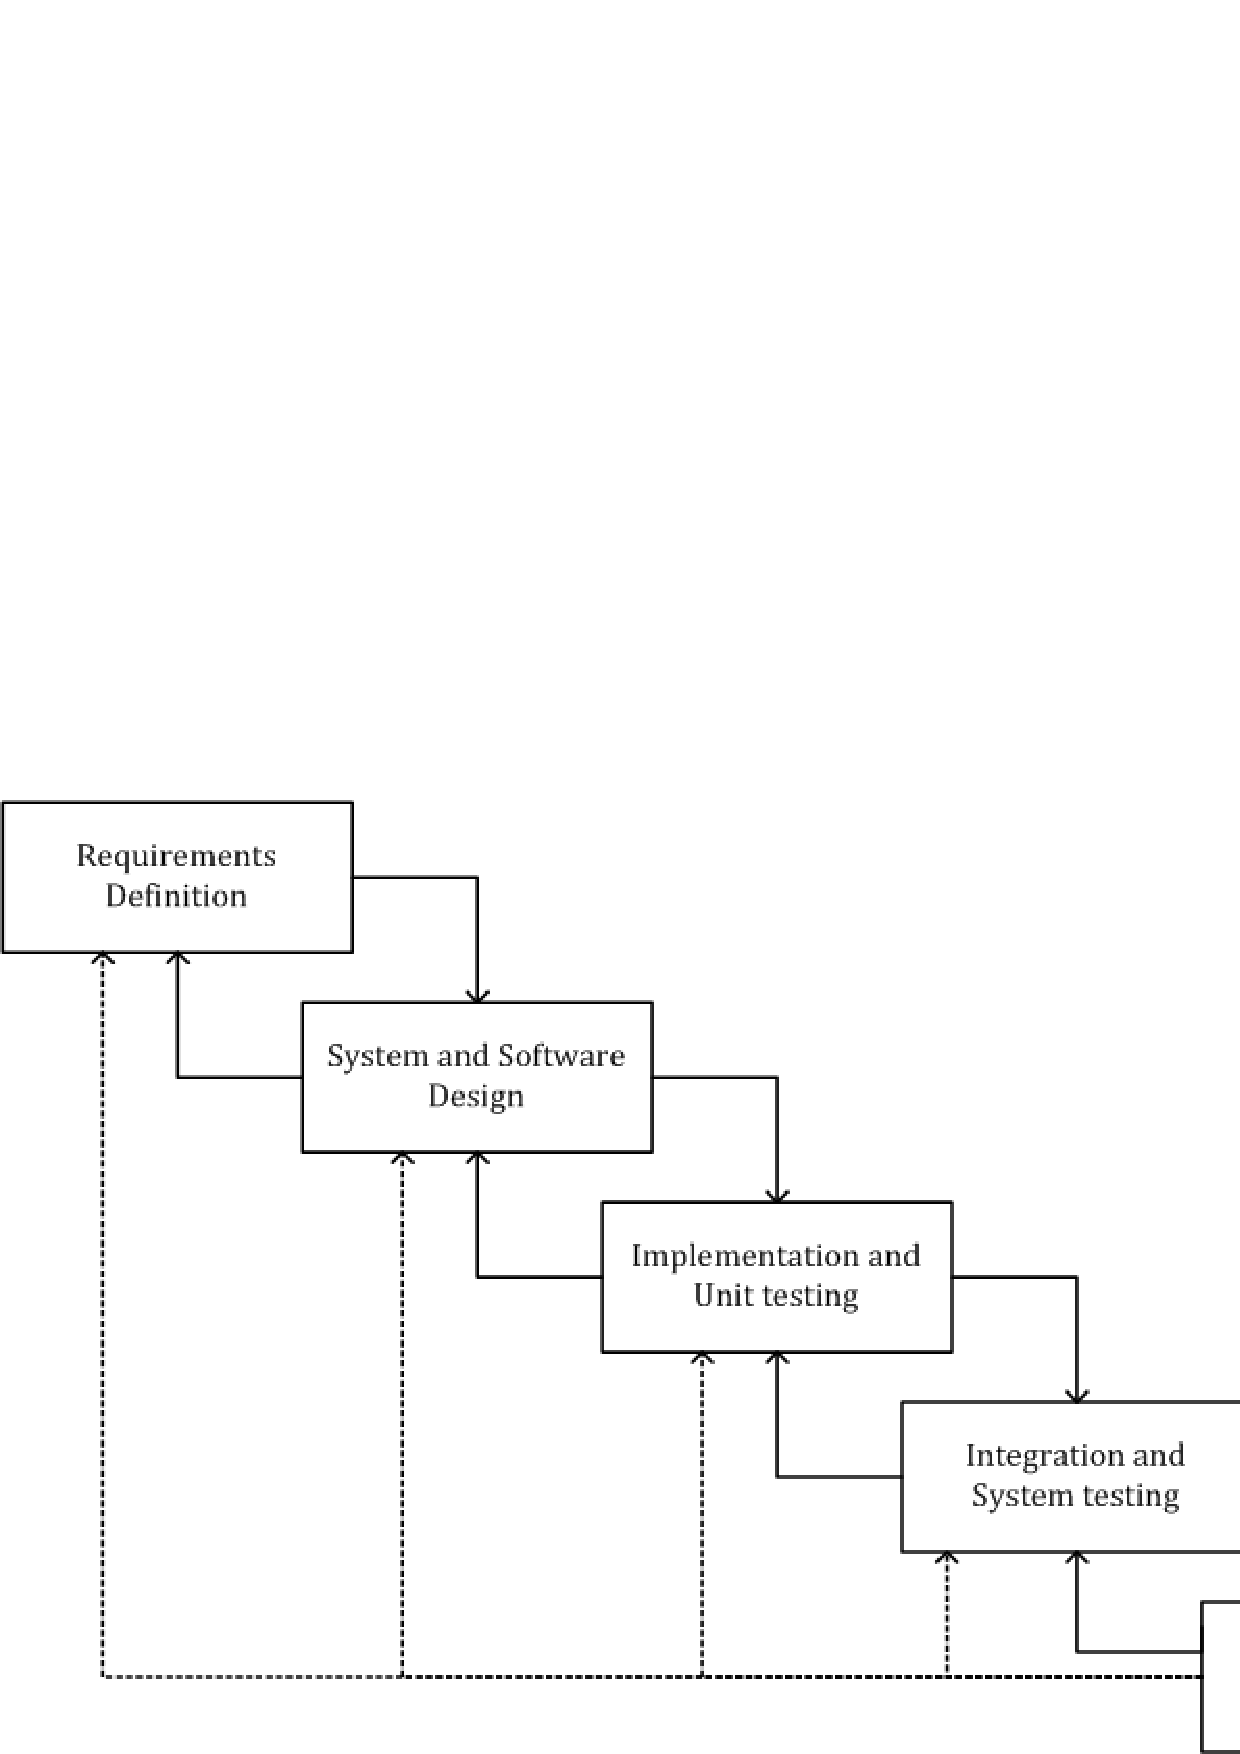
\includegraphics[height=87mm]{model_01_waterfall}
   \caption{The waterfall software development model. Solid lines represent a staged 
      model implementation with no feedback. Dotted lines add a possibilty of 
      iterative transition between adjacent stages. Dashed line show model 
      implementation with feedback \cite{citeulike:9982731}. }
   \label{fig:model_waterfall}
\end{figure}

Waterfall model is an example of a plan-driven process - one must plan and schedule all 
of the activities before their execution. Model has many variations and the approach 
articulated by the model forms the basis of many standards in the software industry.

There is successive and distinct progression of stages in waterfall model; each state 
is well defined and forms the basis for the successive one. In addition to specific 
deliverable, each state producing a document which describes what exactly occurred 
during the stage, providing certain visibility to the processes, and facilitating 
audit. Each state has milestones and deliverables explicitly defined.

Five stages of waterfall model reflect the fundamental development activities:
\begin{enumerate}
 \item \textit{Requirements analysis and definition.} The feasibility study 
is conducted 
and the requirements collected. The system functionality clarified and
documented in details - the requirements specification document - delivered  
and will serve as the system specification. It is assumed that customer's 
expectations are articulated and will not change much throughout the development 
process.
 \item \textit{The system design.} Within this phase requirements for hardware and 
software components defined by the establishing an overall system architecture.
All system modules and their interactions are designed in accordance with 
collected requirements.
 \item \textit{Implementation and unit testing.} The actual code produced, individual 
modules are tested individually. This phase embeds all quality control checks.
 \item \textit{Integration and system testing.} System assembled and once complete, it
is tested and evaluated in actual conditions (alpha tested).
 \item \textit{Delivery and Maintenance.} System is tested by actual customer(s) 
(beta testing). Identified errors are corrected and if found satisfiable, 
software system is installed and put into use. Maintenance involves error correction, 
improvements of system units and enhancements of services if desired.
\end{enumerate}

During transition from stage to stage within the waterfall model, previous state 
should be signed-off - approved to be in finished state. In other 
word, states should not overlap, however in the real life problems often discovered
later on - for example it is often happens that problems with design 
discovered only after implementation is started and so on. In such situation
process returns to the problematic phase and changes are made and reflected in 
the documentation. These iterations are very costly in time and effort and 
usually after a certain number of iterations problematic stages considered 
``frozen'' and development continues. Identified and not resolved issues persist
through the further work and if possible - covered by workarounds, if not - 
they just ignored and system may not perform correctly or lack some functionality 
afterwards.

The big advantage of waterfall model of software development process is that 
it is consistent with other engineering models in terms of general approach, 
its flow and produced documentation. It seems to be manager-friendly too since
it is easy to track the progress against the development plan. The major 
problem with this model is
that within such a specification-based approach stakeholders finding it 
extremely difficult to articulate their requirements in advance and 
that requirements changes are very hard to incorporate after first stages are passed.

In 1988 Boehm revisits waterfall model and after re-stating its fundamental problems 
offers three classes of improved software process models - evolutionary development 
model, the transform model and the spiral model \cite{citeulike:10002126}.

\subsection{Evolutionary development model}
Evolutionary development proposed by McCracken\&Jackson in 1982 \cite{citeulike:3996892}
was among the first reactions to the waterfall model's problems. Instead of moving 
through well-defined stages and producing number of documents, it claims the only
stage - release of extended system capability which is a response to the user 
requirements and is based on the operational experience. Evolutionary paradigm 
is built around early release of the pre-operational product (prototype) and its gradual 
enhancement (evolutional development) through feedback. 

Within the evolutionary development model stakeholders are provided with a somewhat 
functioning software system at the very beginning and their feedback directs all future
software system enhancements. This model perfectly matches the user expectations 
about the software requirements evolution - gradually, through everyday experiences, 
as an opposite to waterfall model upfront requirements collection. 

However, this is what fails in evolutionary development - the new model was found 
stigmatized with weaknesses of the old code-and-fix approach - spaghetti code and 
the lack of formal planning - the exact reasons waterfall model was invented... 
And in addition evolutionary development does not provide any means for identifying 
and fixing early erroneous design decision - instead it encourages working around 
major issues which inevitably creates large expensive to maintain codebase instead 
of re-considering early decisions.


\subsection{Spiral model}
The spiral model reflects the concept in which each of development cycles involves a 
progression addressing the same sequence of steps as in previous level. The figure 
\ref{fig:model_spiral} illustrates the model representation as a spiral according 
to Boehm \cite{citeulike:10002126}. Each loop of this spiral represents a phase of 
software process. Innermost loop concerns the system feasibility study. The second 
loop represents a system requirements definition and system design and so on. 
The radial (Y) dimension represents a cumulative cost of the system up to date, 
while angular dimension represents a loop progress towards completing the current 
spiral loop.

\begin{figure}[tbp]
   \centering
   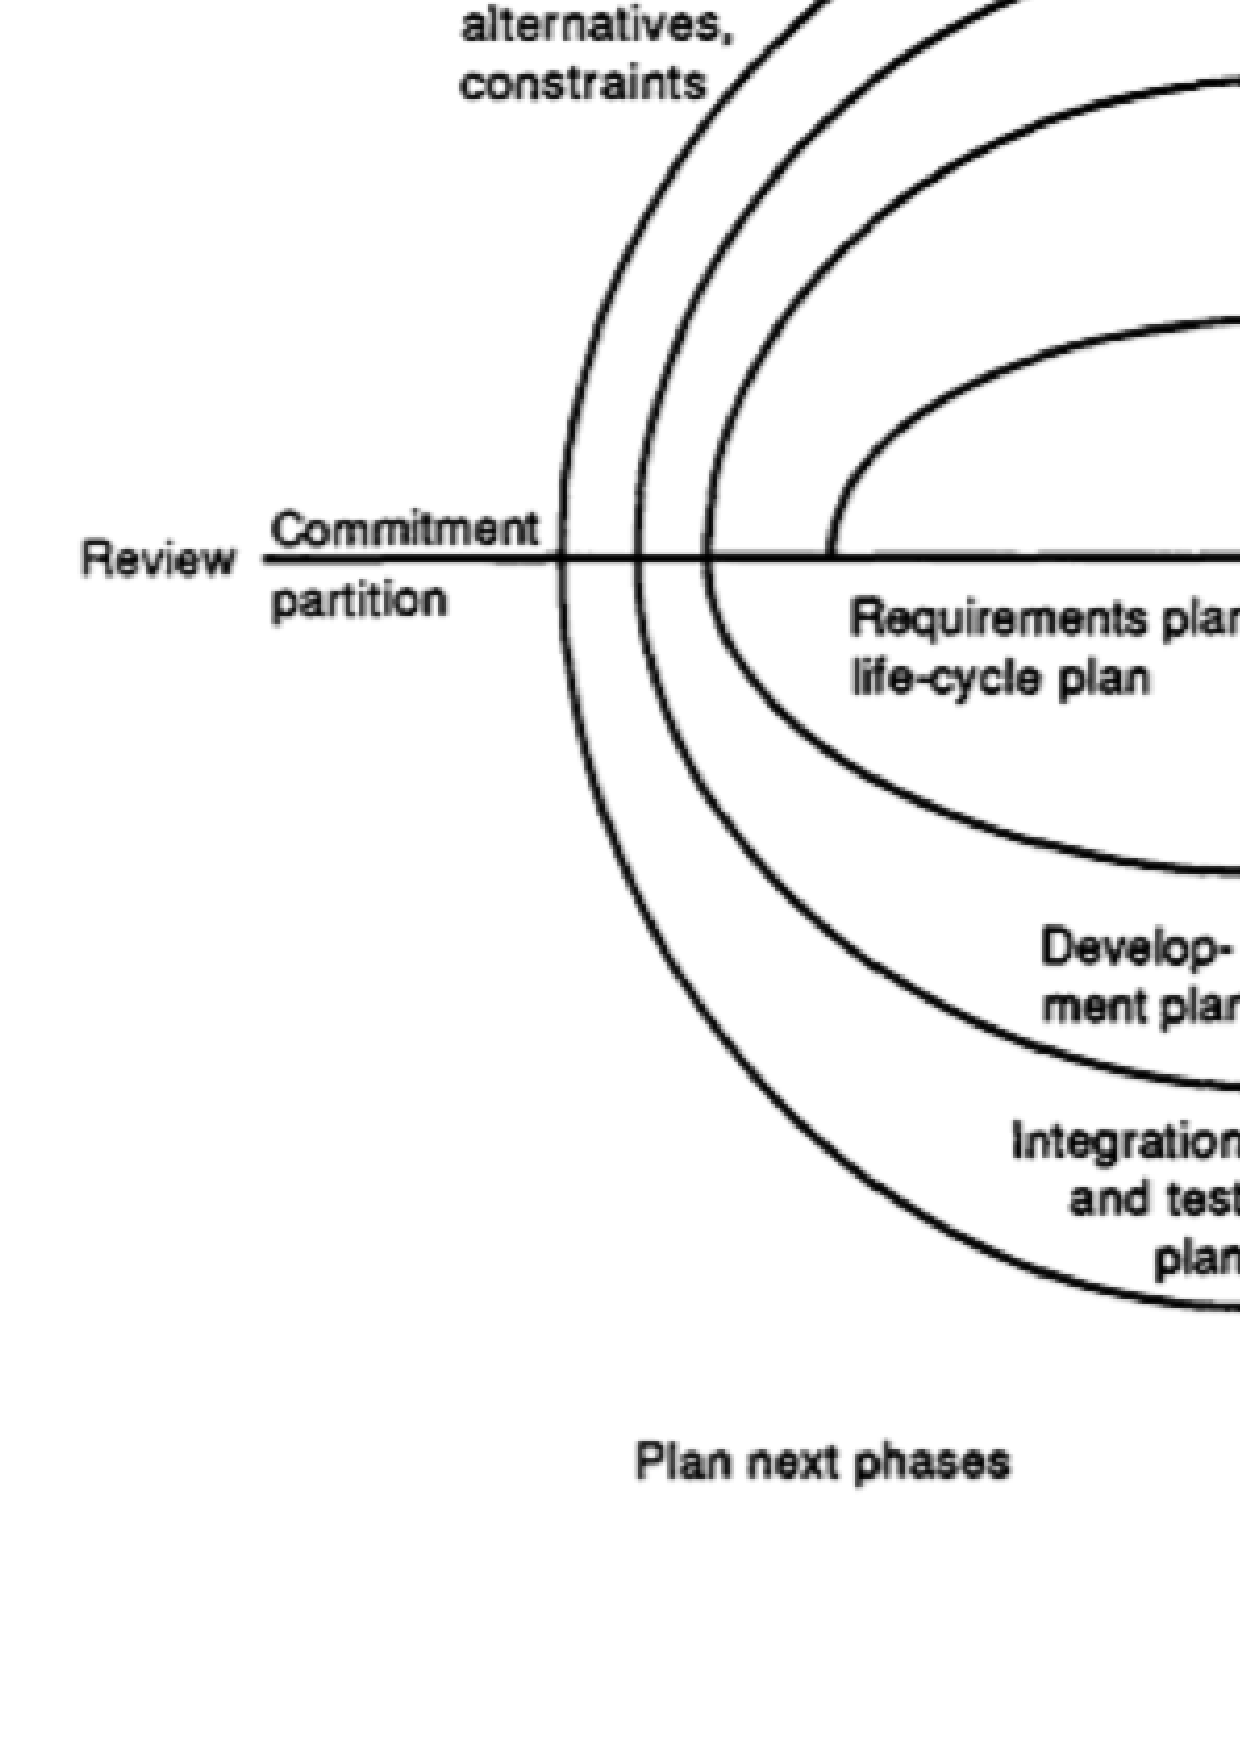
\includegraphics[height=150mm]{model_02_spiral-boehm}
   \caption{The spiral model of software development according to Boehm \cite{citeulike:10002126}. }
   \label{fig:model_spiral}
\end{figure}



\subsection{Cleanroom software engineering}
Another of waterfall model derivatives is a Cleanroom development methodology, which is
a fusion of waterfall model with formal methods approach. 
Following the formal methodology, stages of waterfall model reshaped into 
\begin{enumerate}
 \item \textit{Formal specification} phase, where the software system is presented as 
a state-transition model with input and output. The states of the system and
its transitions (reactions on input) reflect specification and requirements.
 \item \textit{Structured, incremental development} phase. By application of the 
cleanroom methodology the software is partitioned into increments using the 
specification and the development process Within cleanroom
development process only a limited amount of programming constructs allowed,
and the development process is an iterative refinement of specification
\end{enumerate}

1) formal specification phase; 2) incremental, formal development and verification 
, formal methods are a particular kind of mathematically-based techniques for
the specification, development and verification of software and hardware systems

\section{}

It is currently well recognized in the software industry that the process of software development 
is critical to the success of any major development project.
The Institute of Electrical and Electronics Engineers defines software engineering as 
“the application of a systematic, disciplined, quantifiable approach to development, 
operation, and maintenance of software; that is, the application of engineering software”
